
%---------------------------------------%
% Packages arranged by : Tsz Timmy Chan %
%                 Date : May 26th, 2019 % 
%---------------------------------------%

\documentclass{TC}
\usepackage{TCcommon}

\title{TITLE HERE}	% Work Title Here.
\author{Tsz Timmy Chan}	% YOUR NAME HERE 

\usepackage[notes]{TCheader}
\usepackage{TCexamtitle}

\usepackage{setspace}
\linespread{1.5}

%\renewcommand{\benediction}{" " - }
%\renewcommand{\quoteoftheday}{" " \\ - }

\begin{document}
Conducting a Literature Review \parencite{alderman_conducting_2014}:
\begin{itemize}
\item Benefits of a literature review
	\begin{itemize}
	\item Assess current state of research
	\item Identify experts
	\item Identify key questions for further research
	\item Determine methodologies used in past studies of similar topics
	\end{itemize}
\item Steps to conduct a literature review
	\begin{enumerate}
	\item Selecting databases: use library discovery tools. 
		\begin{itemize}[\dangersign]
		\item Some database materials might not be included in discovery tool search
		\item No one tool does it all, "not even Google scholar"
		\item book collections might be excluded
		\item Features available in a particular database might not be available in a discovery tool.
		\item Some discovery tools limit results to what is available through a particular library's collections
		\item Review which databases have been included in the search, and which have not been included.
		\item Go \emph{backwards} by examining the articles in the bibliography to seek past articles, and go \emph{forward} by looking at the "Web of Science" and "Social Sciences Citation Index" to identify article citing the key articles identified in the previous steps \parencite{webster_analyzing_2002}. 
		\end{itemize} 
	\item Formulate an effective search strategy: know the field of that the database, as psychology terms may not work in a human resources management database. Use abstracts of relevant articles to build this list of search terms.
	\item Locate \textit{the actual items} and compose the review. End result should be to discuss the central themes in research and overview of significant studies.
	\item If the dissertation/thesis takes a long time to write, review the literature periodically.
	
	\end{enumerate}
\end{itemize}


\begin{figure}[h]

\begin{mdframed}
\centering
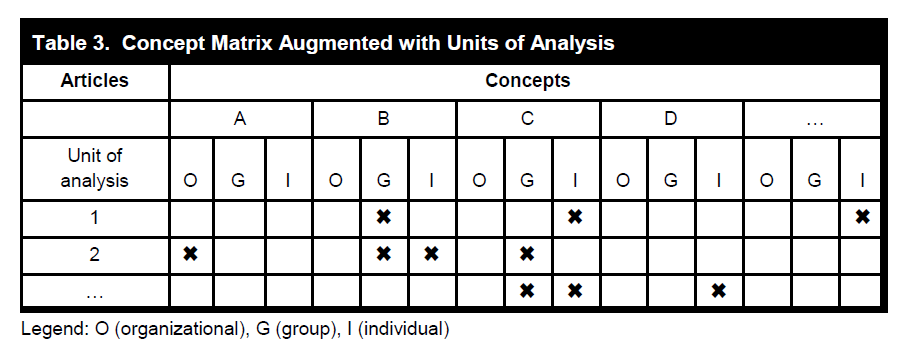
\includegraphics[width=.85\textwidth]{Author_to_Concept_Centric}
\end{mdframed}
\caption{Tool to move from author to concept centric organization \parencite{webster_analyzing_2002}.}\label{fig:Author_to_Concept_Centric}
\end{figure}


Writing a Literature Review \parencite{webster_analyzing_2002}:
\begin{itemize}
\item Types of literature review:
	\begin{enumerate}
	\item Mature topic where an accumulated body of research exists and require analysis and synthesis
	\item Emerging issue that would benefit from exposure to potential theoretical foundations.
	\end{enumerate}
\item Writing a Review Article
\begin{multicols}{2}
	\begin{enumerate}
	\item Beginning: 
		\begin{itemize}
		\item Hook your readers
		\item Provide working definition of key variables
		\item Articulate the paper's contributions such as:
			\begin{itemize}
			\item New theory to analyze or synthesize the existing literature
			\item Point out that little research currently exist
			\item Bring together previously-disparate streams of work
			\item Implications for practice
			\end{itemize}
		\item Identify the contexts in which the theory applies
		\item Support the scope of the search
		\end{itemize}
	\item Organize your literature: Move from author centric to concept centric. \dangersign Sometimes certain concepts are defined differently by different authors based on context or unit of analysis. See \autoref{fig:Author_to_Concept_Centric} for a tool to do such organization.
	\item Stylistics: 
		\begin{itemize}
		\item Tone: summary, so don't be overly critical  
		\item Tense: since this is about the state of the art, choose present tense. Unless you're attributing a concept to a specific person because that may change.
		\end{itemize}
	\item Guiding questions while writing:
		\begin{enumerate}
		\item What's new? (contribution)
		\item So what? (impact)
		\item Why so? (logic)
		\item Well done? (thoroughness)
		\end{enumerate}
	\end{enumerate}

\end{multicols}
\end{itemize}

Lecture Notes:
Types of literature review:
	\begin{itemize}
	\item Scoping (breadth): examining larger field of information.
	\item Rapid Evidence (depth): pick one issue of a part of an area.
	\item Systemic (breadth + depth): EVERYTHING that has been published on the topic. Usually begins with scoping, then identifies areas of focus and do a rapid evidence review on each focus.
		\begin{itemize}
		\item Narrative: Describe the data that is out there, usually as a first step to research projects.
		\item Analytic: Not just review, but also gives interpretation/theory. A good example is the "Who's Not Yet Here" article \parencite{burch_whos_2006}.
		\end{itemize}
	\end{itemize}
Parts of a literature review:
\begin{multicols}{2}
	\begin{itemize}
	\item Purpose
	\item Structure for searching.
		\begin{itemize}	
		\item Inclusion Criteria: "search parameters" to help structure the search and limit it to just relevant articles
			\begin{itemize}
			\item Location
			\item Time span
			\item Types of journals
			\item Databases
			\item Methodologies			
			\end{itemize}
		\item Keywords: most helpful words that are helpful, often the operational definitions; sometimes keywords differ based on time/location. (learning difficulties = UK; whereas intellectual disability = US after 2004, etc.) 
		\end{itemize}
	\item Search Strategy: have one, and know why you're doing this way.
		\begin{itemize}
		\item Boolean:
			\begin{itemize}
			\item uses logical operators \texttt{AND}, \texttt{OR}, \texttt{NOT}.
			\item Use quotes to define text phrases
			\item use asterisk (*) to search for the root of a word.
			\item Advanced search features help \emph{narrow} the search.
			\end{itemize}
		\item "Going backwards", look at the citations until \emph{point of saturation}, i.e., when you keep finding the same articles.
		\item "Go to the source" Begin with an expert - 
		\end{itemize}
	\end{itemize}
\end{multicols}
\textbf{GUIDELINES}
	\begin{multicols}{3}
	\begin{enumerate}
	\item Introduction
	\item Search structure
	\item Findings
	\item Discussion
	\item Conclusion
	\end{enumerate}
	\end{multicols}
Tips
	\begin{itemize}
	\item Pick a reference manager
	\item Choose a citation format
	\item Set up macro/keyboard shortcuts
	\end{itemize}
Theoretical / Conceptual Frameworks
	\begin{itemize}
	\item Theoretical framework explains how theory that is being used works with the research
	\item Helps organize ideas and explain \emph{how} particular frameworks are used.
	\item Operational definition sometimes come with a theoretical/conceptional framework
	\item Uusally in the background section, conception framework might come in during methods also
	\item Disciplinary background may lead to your theoretical framework
	\end{itemize}	

\end{document}
